\chapter{Visualization}
\label{cha:graphics}

\section{Overview}

{\opp} simulations can be run under graphical user interfaces (Tkenv,
Qtenv) that offer visualization and animation in addition to interactive
execution and other features. This chapter deals with model visualization.

{\opp} essentially provides three tools for defining and enhancing
model visualization. \textit{Display strings} is the traditional way:
they define how submodules, connection arrows, and the compound module
containing them will show show up in the graphical user interface.
Display strings can be declared in NED files, and can also be manipulated
programmatically at runtime.

The same user interface area that contains submodules and connections
(we'll refer to it as \textit{canvas}) can also display additional
graphical elements that {\opp} calls \textit{figures}. Using figures, one
can display lines, curves, polygons, images and text items, and anything
that can be built by combining them and applying effects like rotation and
scaling. Like display strings, figures can also be declared in NED files,
but it is generally more useful to create and manipulate them
programmatically. Extra canvas instances can also be created and populated
at runtime.

\textit{3D visualization} is a third possiblity that is completely
different from the previous two. Models have no built-in visualization, 3D
scenes have to be built by the simulation programmer, and they
also appear on a separate GUI area. {\opp}'s 3D visualization support comes
entirely from the OpenGL-based OpenSceneGraph library and its osgEarth
extension. These libraries offer high-level functionality, such as reading
3D model files directly from disk, or displaying maps, 3D terrain or Earth as a
planet using online map and satellite imagery data sources.

Traditionally, when C++ code was needed to enhance visualization, it was
embedded in \ffunc{handleMessage()} functions, enclosed in \ttt{if
(ev.isGUI())} blocks. However, starting from {\opp} version 5.0, such code
can be placed into a dedicated \ffunc{refreshDisplay()} method of modules
(and channels). \ffunc{refreshDisplay()} is not called at all when the
simulation runs under Cmdenv or other non-GUI environment (and thus it has
zero runtime cost), and even when the simulation runs under Qtenv/Tkenv, it
is called much more economically (i.e. exactly when needed and only as
often as needed).

The following sections cover the above topics in more detail.


\section{Display Strings}
\label{sec:ch-graphics:display-strings}

Display strings\index{display strings} are compact textual descriptions
that specify the arrangement and appearance of representations of modules
in graphical user interfaces (currently Tkenv and Qtenv); they control how
the objects (compound modules, their submodules and connections) are
displayed. Display strings are specified in NED's \fprop{@display}
property, and can also be modified at runtime.

Display strings can be used in the following contexts:
\begin{itemize}
  \item \textit{submodules} -- display strings may contain position, arrangement
        (for module vectors), icon, icon color, auxiliary icon, status text,
        communication range (as circle or filled circle), tooltip, etc.
  \item \textit{compound modules, networks} -- display strings can specify
        background color, border color, border width,
        background image, scaling, grid, unit of measurement, etc.
  \item \textit{connections} -- display strings can specify positioning, color,
        line width, line style, text and tooltip
  \item \textit{messages} -- display strings can specify icon, icon color, etc.
\end{itemize}


\subsection{Syntax and Placement}

The display string syntax is a semicolon-separated list of tags.
Each tag consists of a key, an equal sign and a comma-separated list of
arguments:

\begin{ned}
@display("p=100,100;b=60,10,rect,blue,black,2")
\end{ned}

Tag arguments may be omitted both at the end and inside the
parameter list. If an argument is omitted, a sensible default value is used.

\begin{ned}
@display("p=100,100;b=,,rect,blue")
\end{ned}

The following NED sample shows where to place display strings in the code:

\begin{ned}
simple Queue
{
    parameters:
        @display("i=block/queue");
    ...
}

network SimpleQueue
{
    parameters:
        @display("bgi=maps/europe");
    submodules:
        sink: Sink {
            @display("p=273,101");
        }
        ...
    connections:
        source.out --> { @display("ls=red,3"); } --> queue.in++;
}
\end{ned}

\subsection{Display String Inheritance}

Every module and channel object has one single display string object,
which controls its appearance in various contexts. The initial value of
this display string object comes from merging the \fprop{@display}
properties occurring at various places in NED files.
This section describes the rules for merging \fprop{@display} properties
to create the module or channel's display string.

\begin{itemize}
  \item Derived NED types inherit their display string from their base NED type.
  \item Submodules inherit their display string from their type.
  \item Connections inherit their display string from their channel type.
\end{itemize}

The base NED type's display string is merged into the current display string
using the following rules:

\begin{itemize}
  \item If a tag is present in the base display string, but not in the current one
        the whole tag (with all arguments) is added to the current display string.
        (e.g. base: \ttt{"i=icon,red"} current: \ttt{"p=2,4"} result: \ttt{"p=2,4;i=icon,red"})
  \item If a tag is present both in the base and in the current display string
        only tag arguments present in the base, but not in the current display string
        will be copied.
        (e.g. base: \ttt{"b=40,20"} current: \ttt{"b=,30,oval"} result: \ttt{"b=40,30,oval"})
  \item If the current display string contains a tag argument with value "-" (hyphen)
        that argument is treated as empty and will not be inherited from other
        display strings. Requesting the value of this argument will return its the
        default value.
  \item If neither the base display string nor the current one has value for a tag
        a suitable default value will be returned and used.
\end{itemize}

Example of display string inheritance:

\begin{ned}
simple Base {
    @display("i=block/queue"); // use a queue icon in all instances
}

simple Derived extends Base {
    @display("i=,red,60");  // ==> "i=block/queue,red,60"
}

network SimpleQueue {
    submodules:
        submod: Derived {
            @display("i=,yellow,-;p=273,101;r=70");
                     // ==> "i=block/queue,yellow;p=273,101;r=70"
        }
        ...
}
\end{ned}


\subsection{Display String Tags Used in Submodule Context}

The following tags define how a module appears on a graphical user interface
when viewed as a submodule:
\begin{itemize}
  \item{\ttt{b} -- shapes, colors}
  \item{\ttt{i} -- icon}
  \item{\ttt{is} -- icon size}
  \item{\ttt{i2} -- alternate (status) icon placed at the upper right corner of the main icon}
  \item{\ttt{p} -- positioning and layout}
  \item{\ttt{r} -- range indicator}
  \item{\ttt{q} -- queue information text}
  \item{\ttt{t} -- text}
  \item{\ttt{tt} -- tooltip}
\end{itemize}

\subsubsection{Icons}

By default, modules are represented by simple icons.
Using images for the modules is possible with the \ttt{i} tag.
See the \ttt{images} subfolder of your {\opp} installation for possible
icons. The stock images installed with {\opp} have several size variants.
Most of them have very small (vs), small (s), large (l) and
very large (vl) variants. You can specify which variant you want to use with
the \ttt{is} tag.

\begin{ned}
@display("i=block/source;is=l"); // a large source icon from the block icons group
\end{ned}

Sometimes you want to have similar icons for modules, but would like to
make them look a little different to create groups or to reflect status
information about the module. You can easily change the color of an already
existing image. The following example makes the icon 20\% red:

\begin{ned}
@display("i=block/source,red,20")
\end{ned}

\begin{center}
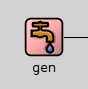
\includegraphics{figures/graphics-itag}
\end{center}

\subsubsection{Status Icon}

If you want to visualize the status of a module, you can use the \ttt{i2}
tag to add a small auxiliary icon. The status icon will appear in the top-right corner
of the main icon. To update the status icon at runtime you can use the
\ffunc{setDisplayString()} method.

\begin{ned}
@display("i=block/queue;i2=status/busy")
\end{ned}

\begin{center}

\includegraphics{figures/graphics-i2tag}
\end{center}

\subsubsection{Shapes}

If you want to have simple but resizable representation for your module, you can use
the \ttt{b} tag to create geometric shapes. Currently, \ttt{oval} and \ttt{rectangle}
are supported:

\begin{ned}
// an oval shape with 70x30 size, red background, black 4 pixel border
@display("b=70,30,oval,red,black,4")
\end{ned}

\begin{center}
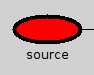
\includegraphics{figures/graphics-btag}
\end{center}

\subsubsection{Positioning, Coordinates}

To define the position of a submodule, use the \ttt{p} tag.
If you do not specify a \ttt{p} tag for your module, the parent module will
automatically choose a position based on a layout algorithm.
The following example will place the module at the given position:

\begin{ned}
@display("p=50,79");
\end{ned}

\begin{note}
The coordinates specified in the \ttt{p}, \ttt{b} or \ttt{r} tags are not necessarily
integers and measured in pixels. You can use the parent module's \ttt{bgs=$pix2unitratio$,$unit$} tag,
to set the scaling parameter and the unit of measurement for your module.
You can specify the ratio between 1 pixel and 1 unit with the \ttt{bgs} tag.
\end{note}

The \ttt{p} tag allows the automatic arrangement of module vectors. They can be
arranged in a row, a column, a matrix or a ring, or you may specify their positions
later at runtime using the \ffunc{setDisplayString()} method. The rest of the arguments
in the \ttt{p} tag depend on the layout type:

\begin{itemize}
  \item \ttt{row -- p=100,100,r,$deltaX$} (A row of modules with $deltaX$ units between the modules)
  \item \ttt{column -- p=100,100,c,$deltaY$} (A column of modules with $deltaX$ units between the modules)
  \item \ttt{matrix -- p=100,100,m,$noOfCols$,$deltaX$,$deltaY$} (A matrix with $noOfCols$ columns.
            $deltaX$ and $deltaY$ units between rows and columns)
  \item \ttt{ring -- p=100,100,ri,$rx$,$ry$} (A ring (oval) with $rx$ and $ry$ as the horizontal and vertical radius.)
  \item \ttt{exact (default) -- p=100,100,x,$deltaX$,$deltaY$} (Place each module at $(100+deltaX, 100+deltaY)$.
            The coordinates are usually set at runtime.)
\end{itemize}

A matrix layout for a module vector:

\begin{ned}
@display("p=,,m,4,50,50");
\end{ned}

\begin{figure}[htbp]
  \begin{center}
    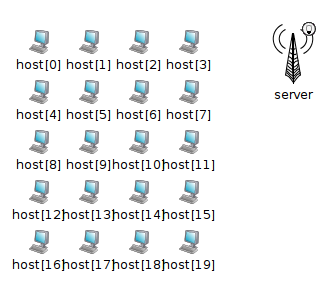
\includegraphics{figures/graphics-ptag}
    \caption{Matrix arrangement using the $p$ tag}
    \label{fig:graphics-ptag}
  \end{center}
\end{figure}

\subsubsection{Wireless Range}
In wireless simulations it is very useful to show some kind of range
around your module. This can be an interference range, transmission range
etc. The following example will place the module at a given position,
and draw a circle with a 90-unit radius around it as a range indicator:

\begin{ned}
submodules:
    ap: AccessPoint {
        @display("p=50,79;r=90");
    }
\end{ned}

\begin{figure}[htbp]
  \begin{center}
    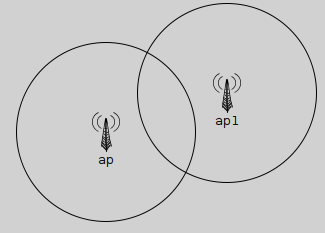
\includegraphics{figures/graphics-rtag}
    \caption{Range indicator using the $r$ tag}
    \label{fig:graphics-rtag}
  \end{center}
\end{figure}

\subsubsection{Queue Length}

If a module contains a queue object (\cclass{cQueue}), it is possible to
let the graphical user interface display the queue length next to the
module icon. To achieve that, specify the queue object's name (the string
set via the \ffunc{setName()} method) in the \ttt{q} display string tag.
{\opp} will find the queue object by traversing the object tree inside
the module.

For example, if the module contains an \cclass{cQueue} object named
\ttt{"procqueue"}, you can can specify \ttt{q=procqueue} in the display
string.

\begin{ned}
@display("q=procqueue");
\end{ned}

\begin{center}
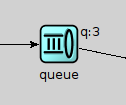
\includegraphics{figures/graphics-qtag}
\end{center}

\subsubsection{Text and Tooltip}

You can add a text description to any module using the \ttt{t}
(displayed along the module) or \ttt{tt} tag (displayed as a tooltip).
The following example displays a short text string along with the module
and adds a tooltip text string that can be seen by hovering over
them module with the mouse.

\begin{ned}
@display("t=Packets sent: 18;tt=Additional tooltip information");
\end{ned}

\begin{center}
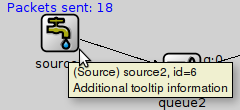
\includegraphics{figures/graphics-ttag}
\end{center}

\begin{note}
  The \ttt{t} and \ttt{tt} tags, when set at runtime, can be used to display
  various information about the module's state. The \ffunc{setTagArg()} method
  of \cclass{cDisplayString} can be used to update the text:

  \begin{cpp}
char buf[64];
sprintf(buf, "sent: %d, rcvd: %d", numPkSent, numPkReceived);
getDisplayString().setTagArg("t", 0, buf);
  \end{cpp}

\end{note}

For a detailed descripton of the display string tags, check
Appendix \ref{cha:display-string-tags}.

\subsection{Display String Tags Used in Module Background Context}

The following tags describe what a module looks like when opened in
a graphical user interface. They mostly deal with the module background.

\begin{itemize}
  \item \ttt{bgi} -- background image
  \item \ttt{bgtt} -- tooltip above the background
  \item \ttt{bgg} -- background grid
  \item \ttt{bgl} -- child layout
  \item \ttt{bgb} -- background size, color, border
  \item \ttt{bgs} -- scaling of background coordinates
  \item \ttt{bgp} -- background coordinate offset
\end{itemize}

The \ttt{bgs} tag makes it possible to use a physical unit of measurement,
(e.g. kilometers) for coordinates. \ttt{bgs} arguments include a pixel-per-unit
factor (for mapping coordinates to the screen), and a unit name. When \ttt{bgs}
is present, all coordinates (including submodule coordinates) are interpreted
in the given unit of measurement. When combined with the \ttt{bgi} (background
image) and \ttt{bgg} (grid) tags, it is possible to display maps.

The following example demonstrates the use the of module background tags.
The coordinates are given in km (SI unit). The \ttt{bgs=$pixelsperunit$,$unit$}
specifies pixel/unit ratio, i.e. 1km is 0.075 pixel on the screen.
The whole area is 6000x4500km (\ttt{bgb=}) and the map of Europe is used as a
background and stretched to fill the module background.
A light grey grid is drawn with a 1000km distance between major ticks,
and 2 minor ticks per major tick (\ttt{bgg=tickdistance,minorpermajorticks,color}).
See Figure \ref{fig:graphics-bgtags}.

\begin{ned}
network EuropePlayground
{
    @display("bgb=6000,4500;bgi=maps/europe,s;bgg=1000,2,grey95;bgs=0.075,km");
\end{ned}

\begin{figure}[htbp]
  \begin{center}
    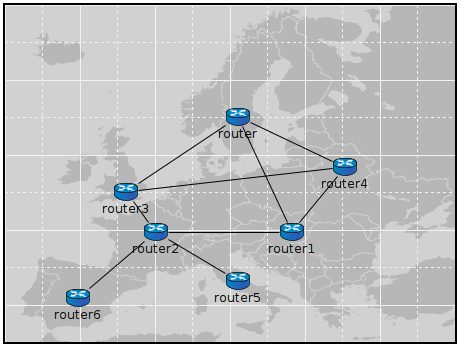
\includegraphics{figures/graphics-bgtags}
    \caption{Background grid, scaling and image}
    \label{fig:graphics-bgtags}
  \end{center}
\end{figure}

After specifying the above \ttt{bgs} tag, all your submodule coordinates will be treated as if
they were specified in km.

For a detailed descripton of the display string tags, check
Appendix \ref{cha:display-string-tags}.

\subsection{Connection Display Strings}

Connections may also have display strings. Connections inherit the
display string property from their channel types, in the same way as
submodules inherit theirs from module types. The default display
strings are empty.

Connections support the following tags:
\begin{itemize}
  \item{\ttt{ls} -- line style and color}
  \item{\ttt{t} -- text}
  \item{\ttt{tt} -- tooltip}
  \item{\ttt{m} -- orientation and positioning}
\end{itemize}

Example of a thick, red connection:
\begin{ned}
source1.out --> { @display("ls=red,3"); } --> queue1.in++;
\end{ned}

\begin{center}
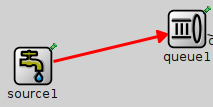
\includegraphics{figures/graphics-lstag}
\end{center}

\begin{note}
If you want to hide a connection, specify zero line width in the display
string (\ttt{"ls=,0"}).
\end{note}

For a detailed descripton of the display string tags, check
Appendix \ref{cha:display-string-tags}.

\subsection{Message Display Strings}

Message display strings affect how messages are shown during animation.
By default, they are displayed as a small filled circle, in one of
8 basic colors (the color is determined as \textit{message kind modulo 8}),
and with the message class and/or name displayed under it.
The latter is configurable in the Options dialog of Tkenv and Qtenv,
and message kind dependent coloring can also be turned off there.

\subsubsection{Specifying Message Display Strings}

Message objects do not store a display string by default, but you can redefine
the \cclass{cMessage}'s \ffunc{getDisplayString()} method and make it return
one.

Example of using an icon to represent a message:

\begin{cpp}
const char *CustomPacket::getDisplayString() const
{
    return "i=msg/packet;is=vs";
}
\end{cpp}

Alternatively, you can add the field \ffunc{displayString} to your message
definition (.msg file), and the message compiler will automatically generate
\ffunc{setDisplayString()} and \ffunc{getDisplayString()} methods for you:

\begin{msg}
message Job
{
    string displayString = "i=msg/package_s,kind";
...
\end{msg}

\subsubsection{Message Display String Tags}

The following tags can be used in message display strings:
\begin{itemize}
  \item{\ttt{b} -- shapes, colors}
  \item{\ttt{i} -- icon}
  \item{\ttt{is} -- icon size}
\end{itemize}

Using a small red box icon to represent the messages:

\begin{ned}
@display("i=msg/box,red;is=s");
\end{ned}

Messages will be represented by a 15x15 rectangle with white background.
Their border color will depend on the \ttt{messageKind} property of the message.

\begin{ned}
@display("b=15,15,rect,white,kind,5");
\end{ned}

\begin{note}
   In message display strings you may use the word \ttt{kind} as a special color.
   This virtual color depends on the \ttt{messageKind} field in the message.
\end{note}

%FIXME more examples, WITH EXPLANATIONS


\subsection{Parameter Substitution}

Parameters of the module or channel containing the
display string can be substituted into the display string
with the \ttt{\$parameterName} notation:

Example:

\begin{ned}
simple MobileNode
{
    parameters:
        double xpos;
        double ypos;
        string fillColor;
        // get the values from the module parameters xpos,ypos,fillcolor
        @display("p=$xpos,$ypos;b=60,10,rect,$fillColor,black,2");
}
\end{ned}

\subsection{Colors}
\label{sec:ch-graphics:colors}

\subsubsection{Color Names}

Any valid Tk color specification is accepted: English color names
(blue, lightgrey, wheat) or \textit{\#rgb}, \textit{\#rrggbb} format
(where \textit{r},\textit{g},\textit{b} are hex digits).

It is also possible to specify colors in HSB (hue-saturation-brightness) as
\textit{@hhssbb} (with \textit{h}, \textit{s}, \textit{b} being hex digits).
HSB makes it easier to scale colors e.g. from white to bright red.

You can produce a transparent background by specifying a hyphen (\textit{"-"})
as background color.

In message display strings, \ttt{kind} can also be used as a special color name.
It will map to a color depending on the message kind.
(See the \ffunc{getKind()} method of \cclass{cMessage}.)

\subsubsection{Icon Colorization}

The \ttt{"i="} display string tag allows for colorization of icons.
It accepts a target color and a percentage as the degree of colorization.
Percentage has no effect if the target color is missing.
Brightness of the icon is also affected -- to keep the original brightness,
specify a color with about 50\% brightness (e.g. \#808080 mid-grey,
\#008000 mid-green).

Examples:

\begin{itemize}
  \item \ttt{"i=device/server,gold"} creates a gold server icon
  \item \ttt{"i=misc/globe,\#808080,100"} makes the icon greyscale
  \item \ttt{"i=block/queue,white,100"} yields a "burnt-in" black-and-white icon
\end{itemize}

Colorization works with both submodule and message icons.


\subsection{Icons}
\label{sec:ch-graphics:icon-library}

\subsubsection{The Image Path}

In the current {\opp} version, module icons are PNG or GIF files. The icons shipped
with {\opp} are in the \ttt{images/} subdirectory. The IDE, Tkenv and Qtenv all
need the exact location of this directory to be able to load the icons.

Icons are loaded from all directories in the \textit{image path},
a semicolon-separated list of directories.
The default image path is compiled into Tkenv and Qtenv with the value
\ttt{"\textit{omnetpp-dir}/images; ./images;./bitmaps"} -- which will work fine
as long as you don't move the directory, and you will also be able to
load more icons from the \ttt{images/} subdirectory of the current
directory. As users typically run simulation models from the model's
directory, this practically means that custom icons placed in the
\ttt{images/} subdirectory of the model's directory are automatically
loaded.

The compiled-in image path can be overridden with the \ttt{OMNETPP\_IMAGE\_PATH}
environment variable. The way of setting environment variables is system
specific: in Unix, if you are using the bash shell, adding a line

\begin{commandline}
export OMNETPP_IMAGE_PATH="/home/you/images;./images"
\end{commandline}

to \ttt{\textasciitilde/.bashrc} or \ttt{\textasciitilde/.bash\_profile} will do;
on Windows, environment variables can be set via the \textit{My Computer --> Properties} dialog.

You can extend the image path from \ffilename{omnetpp.ini} with the
\ttt{image-path} option, which is prepended to the environment
variable's value.

\begin{inifile}
[General]
image-path = "/home/you/model-framework/images;/home/you/extra-images"
\end{inifile}


\subsubsection{Categorized Icons}

Since {\opp} 3.0, icons are organized into several categories, represented
by folders. These categories include:

\begin{itemize}
  \item block/ - icons for subcomponents (queues, protocols, etc).
  \item device/ - network devices: servers, hosts, routers, etc.
  \item abstract/ - symbolic icons for various devices
  \item misc/ - node, subnet, cloud, building, town, city, etc.
  \item msg/ - icons that can be used for messages
\end{itemize}

Old (pre-3.0) icons are in the \ttt{old/} folder.

The IDE, Tkenv and Qtenv now load icons from subdirectories of all directories
of the image path, and these icons can be referenced from display strings
by naming the subdirectory (subdirectories) as well:
\ttt{"subdir/icon"}, \ttt{"subdir/subdir2/icon"}, etc.

For compatibility, if the display string contains an icon without
a category (i.e. subdirectory) name, {\opp} attempts to load it from "old/icon" as well.

\subsubsection{Icon Size}

Icons come in various sizes: normal, large, small, very small. Sizes are
encoded into the icon name's suffix: \ttt{\_vl}, \ttt{\_l}, \ttt{\_s}, \ttt{\_vs}.
In display strings, one can either use the suffix (\ttt{"i=device/router\_l"}),
or the \ttt{"is}" (\textit{icon size}) display string tag (\ttt{"i=device/router;is=l"}),
but not both at the same time (we recommend using the \ttt{is} tag whenever possible).

%The word "layouting" doesn't appear in the English dictionary, although it seems to appear
%  commonly in technical articles, etc. on the web. Up to this point, I have changed all
%  uses of layouting to layout, but I will leave it up to you to decide which one to use.
%  It sounds wrong to me, but it may be an acceptable usage in your particular domain.

\subsection{Layouting}
\label{sec:ch-graphics:layouting}

{\opp} implements an automatic layouting feature, using
a variation of the SpringEmbedder algorithm. Modules which have
not been assigned explicit positions via the \ttt{"p="} tag will be
automatically placed by the algorithm.

SpringEmbedder is a graph layouting algorithm based on a physical model.
Graph nodes (modules) repel each other like electric charges
of the same sign, and connections are sort of springs which try
to contract and pull the nodes they're attached to together. There is also friction
built in, in order to prevent oscillation of the nodes. The layouting algorithm
simulates this physical system until it reaches equilibrium
(or times out). The physical rules above have been slightly tweaked
to achieve better results.

The algorithm doesn't move any module which has fixed coordinates.
Predefined row, matrix, ring or other arrangements (defined
via the 3rd and further args of the \ttt{"p="} tag) will be preserved --
you can think about them as if those modules were attached
to a rigid framework so that they can only move as one unit.

Caveats:

\begin{itemize}
  \item If the full graph is too big after layouting, it is scaled
    back so that it fits on the screen, \textit{unless it contains
    any fixed-position module}. (For obvious reasons: if there is a module
    with manually specified position, we don't want to move that one).
    To prevent rescaling, you can specify a sufficiently large bounding
    box in the background display string, e.g. \ttt{"b=2000,3000"}.
  \item Size is ignored by the present layouter, so longish modules
    (such as an Ethernet segment) may produce funny results.
  \item The algorithm is prone to produce erratic results, especially
    when the number of submodules is small, or when using predefined
    (matrix, row, ring, etc) layouts. The "Re-layout" toobar button
    can then be very useful. Larger networks usually produce
    satisfactory results.
  \item The algorithm is starting from random positions.
     To get the best results you may experiment with
    different seeds by specifying them using the \ttt{bgl=\textit{seed}}
    display string tag.
\end{itemize}

\subsection{Changing Display Strings at Runtime}

It is often useful to manipulate the display string at runtime.
Changing colors, icon, or text may convey status change, and
changing a module's position is useful when simulating mobile
networks.

Display strings are stored in \cclass{cDisplayString} objects inside
channels, modules and gates. \cclass{cDisplayString} also lets you
manipulate the string.

To get a pointer to the \cclass{cDisplayString} object, you can call
the components's \ffunc{getDisplayString()} method:

\begin{cpp}
// Setting a module's position, icon and status icon:
cDisplayString& dispStr = getDisplayString();
dispStr.parse("p=40,20;i=device/cellphone;i2=status/disconnect");
\end{cpp}

\begin{note}
The connection display string is stored in the channel object, but it
can also be accessed via the source gate of the connection.
\end{note}

\begin{cpp}
// Setting an outgoing connection's color to red:
cDisplayString& connDispStr = gate("out")->getDisplayString();
connDispStr.parse("ls=red");
\end{cpp}

\begin{note}
In {\opp} 3.x, to manipulate the appearance of a compound module you had to use
the \ffunc{backgroundDisplayString()} method. This method is no longer
available from {\opp} 4.0 on, because there is no separate background display string.
Use the \ffunc{getDisplayString()} method instead with the background
specific tags, i.e. those starting with \ttt{bg}.
\end{note}

\begin{cpp}
// Setting module background and grid with background display string tags:
cDisplayString& parentDispStr = getParentModule()->getDisplayString();
parentDispStr.parse("bgi=maps/europe;bgg=100,2");
\end{cpp}

As far as \cclass{cDisplayString} is concerned, a display string
(e.g. \ttt{"p=100,125;i=cloud"}) is a string that consist of several
\textit{tags} separated by semicolons, and each tag has a \textit{name}
and after an equal sign, zero or more \textit{arguments} separated by commas.

The class facilitates tasks such as finding out what tags a display string
has, adding new tags, adding arguments to existing tags,
removing tags or replacing arguments. The internal storage method allows
very fast operation; it will generally be faster than direct string manipulation.
The class doesn't try to interpret the display string in any way, nor does
it know the meaning of the different tags; it merely parses the string
as data elements separated by semicolons, equal signs and commas.

An example:

\begin{cpp}
dispStr.parse("a=1,2;p=alpha,,3");
dispStr.insertTag("x");
dispStr.setTagArg("x",0,"joe");
dispStr.setTagArg("x",2,"jim");
dispStr.setTagArg("p",0,"beta");
EV << dispStr.str();  // result: "x=joe,,jim;a=1,2;p=beta,,3"
\end{cpp}

\subsection{Bubbles}

Modules can display a transient bubble with a short message (e.g. "Going
down" or "Connection estalished") by calling the \ffunc{bubble()} method of
\cclass{cComponent}. The method takes the string to be displayed as a
\ttt{const char *} pointer.

An example:
\begin{cpp}
bubble("Collision! (2 frames)");
\end{cpp}

\begin{center}
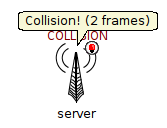
\includegraphics{figures/graphics-bubble}
\end{center}

If the module contains a lot of code that modifies the display string or
displays bubbles, it is recommended to make these calls conditional
on \ffunc{hasGUI()}. The \ffunc{hasGUI()} method returns \textit{false}
if the simulation is run under Cmdenv, so one can make the code skip
potentially expensive display string manipulation.

Better:
\begin{cpp}
if (hasGUI())
    bubble("Going down!");
\end{cpp}



\section{The Canvas}
\label{sec:ch-graphics:canvas}

\subsection{Overview}

The canvas is the 2D drawing API of {\opp}. Using the canvas, one can
display lines, curves, polygons, images, text items and their combinations,
using colors, transparency, geometric transformations, antialiasing and
more. Drawings created with the canvas API can be viewed when the simulation
is run under a graphical user interface (Tkenv or Qtenv).

Use cases for the canvas API include displaying textual annotations,
status information, live statistics in the form of plots, charts, gauges,
counters, etc. Other types of simulations may call for different types of
graphical presentation. For example, in mobile and wireless simulations,
the canvas API can be used to draw the scene including a background (like a
street map or floor plan), mobile objects (vehicles, people), obstacles
(trees, buildings, hills), antennas with orientation, and also extra
information like connectivity graph, movement trails, individual
transmissions and so on.

An arbitrary number of drawings (canvases) can be created, and every module
already has one by default. A module's default canvas is the one on which
the module's submodules and internal connections are also displayed, so the
canvas API can be used to enrich the default, display string based
presentation of a compound module.

{\opp} calls the items that appear on a canvas \textit{figures}. The
corresponding C++ types are \cclass{cCanvas} and \cclass{cFigure}. In fact,
\cclass{cFigure} is an abstract base class, and different kinds of figures
are represented by various subclasses of \cclass{cFigure}.

Figures can be declared statically in NED files using \fprop{@figure}
properties, and can also be accessed, created and manipulated
programmatically at runtime.


\subsection{Creating, Accessing and Viewing Canvases}

A canvas is represented by the \cclass{cCanvas} C++ class. A module's
default canvas can be accessed with the \ffunc{getCanvas()} method of
\cclass{cModule}. For example, a toplevel submodule can get hold of the
network's canvas with the following line:

\begin{cpp}
cCanvas *canvas = getParentModule()->getCanvas();
\end{cpp}

Using the canvas pointer, it is possible to check what figures it
contains, add new figures, manipulate existing ones, and so on.

New canvases can be created by simply creating new \cclass{cCanvas}
objects, like so:

\begin{cpp}
cCanvas *canvas = new cCanvas("liveStatistics"); // arbitrary name string
\end{cpp}

To view the contents of these additional canvases in Tkenv or Qtenv, one
needs to navigate to the canvas' owner object (which will usually be the
module that created the canvas), view the list of objects it contains, and
double-click the canvas in the list. Giving meaningful names to extra
canvas objects like in the example above can simplify the process of
locating them in the Tkenv/Qtenv GUI.


\subsection{Figure Classes}

The base class of all figure classes is \cclass{cFigure}. The class hierarchy
is shown below.

\begin{figure}[htbp]
  \begin{center}
    \includegraphics{figures/figure-inheritance}
    \caption{cFigure class hierarchy}
  \end{center}
\end{figure}

In subsequent sections, we'll first describe features that are common
to all figures, then we'll briefly cover each figure class. Finally,
we'll look into how one can define new figure types.

\begin{note}
Figures are only data storage classes. The real drawing code is inside
Tkenv/Qtenv; it might involve a parallel data structure, figure renderer classes, etc.
When an inspector is not open, these things don't exist. Therefore, data flow
is only one-directional -- figures affect the rendered image, but figures
cannot access e.g. the actual bounding box of a text just drawn.
\end{note}


\subsection{Figure Hierarchy}

Figures on a canvas form a hierarchy. The canvas has a \textit{root
figure}, and all toplevel figures in the canvas are children of the root
figure. In addition, any figure may contain further figures as children.
(That is, \textit{child list} is the built-in property of \cclass{cFigure},
not of a specific subclass like \cclass{cGroupFigure}.)

Every figure also has a name string, inherited from \cclass{cNamedObject}.
Putting it together with the figure hierarchy, this means that every figure
also has a \textit{hierarchical name}. It consists of the names of figures
in the path from the root figure down to the the figure, joined with dots.
(The name of the root figure itself is omitted.)

You can get the root figure of the canvas with the \ffunc{getRootFigure()}
member function, but that is usually unnecessary, because the
\cclass{cCanvas}, like \cclass{cFigure}, has methods for accessing and
manipulating its child figures directly.

You can add a child figure \ffunc{addFigure()}. It has two flavours: one
for appending, and one for inserting at a numeric position. The order of
children is important because it also denotes Z-order. Z-order comes into
play when children are overlapping on the screen: the first child will be
the bottom-most one, and the last child the topmost one (think of it like
drawing order). The methods \ffunc{addFigureAbove()} and
\ffunc{addFigureBelow()} allows one to insert a figure into the child list
relative to an existing child figure.

Child figures can be accessed by name (\ffunc{getFigure(const char *)}), or
enumerated by index in the child list (\ffunc{getFigure(int)},
\ffunc{getNumFigures()}). You can obtain the index of a child figure using
\ffunc{findFigure()}.

The following code illustrates these methods:

\begin{cpp}
// print the names of child figures above "cloud" in Z-order
// (in the code, 'parent' can be either a canvas or a figure):
cFigure *cloudFigure = parent->getFigure("cloud");
if (cloudFigure) {
    int cloudPos = parent->findFigure(cloudFigure);
    for (int i = cloudPos+1; i < parent->getNumFigures(); i++)
        EV << parent->getFigure(i)->getName() << endl;
}
\end{cpp}

It is also possible to locate a figure by its hierarchical name
(\ffunc{getFigureByPath()}), and to find figure by its (non-hierarchical)
name anywhere in a figure subtree (\ffunc{findFigureRecursively()}).

To remove a figure from the child list, use \ffunc{removeFigure()} with
either the figure's pointer or its index in the child list.


\subsection{Creating and Manipulating Figures from NED and C++}

As mentioned earlier, figures can also be defined in the NED file, so they
don't always need to be created programmatically. This possibility is
useful for creating static backgrounds or statically defining placeholders
for dinamically displayed items, among others. Figures defined from NED can
be accessed and manipulated from C++ code just like dynamically created
ones.

Figures are defined in NED by adding \fprop{@figure} properties to a module definition.
The hierarchical name of the figure goes into the property index, that is, in
square brackets right after \ttt{@figure}. The parent of the figure must
already exist, that is, when defining \ttt{foo.bar.baz}, both \ttt{foo} and
\ttt{foo.bar} must have already been defined (in NED).

Type and various attributes of the figure go into property body, as
\textit{key-valuelist} pairs. The \ttt{type=line} creates a
\cclass{cLineFigure}, \ttt{type=rectangle} creates a
\cclass{cRectangleFigure}, \ttt{type=text} creates a \cclass{cTextFigure},
and so on; the list of accepted types is given in appendix
\ref{cha:figure-definitions}. Further attributes largely correspond to
getters and setters of the C++ class denoted by the \ttt{type} attribute.

The following example creates a green rectangle and the text
\textit{"placeholder"} in it in NED, and the subsequent C++ code changes
the same text to \textit{"Hello World!"}.

NED part:

\begin{ned}
module Foo
{
    @display("bgb=800,500");
    @figure[box](type=rectangle; coords=10,50; size=200,100; fillColor=green);
    @figure[box.txt](type=text; coords=20,80; text=placeholder);
}
\end{ned}

And the C++ part:

\begin{cpp}
// we assume this code runs in a submodule of the above "Foo" module
cCanvas *canvas = getParentModule()->getCanvas();

// obtain the figure pointer by hierarchical name, and change the text:
cTextFigure *textFigure = dynamic_cast<cTextFigure *>(
                              canvas->getFigureByPath("box.txt"));
textFigure->setText("Hello World!");
\end{cpp}

%% In addition to \ttt{type}, there are some more special attributes
%% (\ttt{visible}, \ttt{tags}, \ttt{transform}, \ttt{childZ})




\subsection{Transforms}

One of the most powerful features of the Canvas API is being able to assign
geometric transformations to figures. {\opp} uses 2D homogeneous
transformation matrices, which are able to express affine transforms such
as translation, scaling, rotation and skew (shearing). The
transformation matrix used by {\opp} has the following format:

\[ T = \left( \begin{array}{ccc}
a & c & t_1 \\
b & d & t_2 \\
0 & 0 & 1 \end{array} \right)\]

In a nutshell, given a point with its $(x, y)$ coodinates, one can obtain the
transformed version of it by multiplying the transformation matrix by the
$(x \ y \ 1)$ column vector (a.k.a. homogeneous coordinates), and dropping the
third component:

\[ \left( \begin{array}{c} x' \\ y' \\ 1 \end{array} \right)
 = \left( \begin{array}{ccc}
a & c & t_1 \\
b & d & t_2 \\
0 & 0 & 1 \end{array} \right)
\left( \begin{array}{c} x \\ y \\ 1 \end{array} \right)
\]

The result is the point $(ax+cy+t_1, bx+dy+t_2)$. As one can deduce, $a$,
$b$, $c$, $d$ are responsible for rotation, scaling and skew, and $t_1$ and
$t_2$ for translation. Also, transforming a point by matrix $T_1$ and then by
$T_2$ is equivalent to transforming the point by the matrix $T_2 T_1$ due to
the associativity of matrix multiplication.


\subsubsection{cFigure::Transform}

Transformation matrices are represented in {\opp} by the \cclass{cFigure::Transform}
class.

A \cclass{cFigure::Transform} transformation matrix can be initialized in
several ways. First, it is possible to assign its \ttt{a}, \ttt{b},
\ttt{c}, \ttt{d}, \ttt{t1}, \ttt{t2} members directly (they are public), or
via a six-argument constructor. However, it is usually more convenient to
start from the identity transform (as created by the default constructor), and
invoke one or more of its several \ffunc{scale()}, \ffunc{rotate()},
\ffunc{skewx()}, \ffunc{skewy()} and \ffunc{translate()} member functions.
They update the matrix to (also) perform the given operation (scaling,
rotation, skewing or translation), as if left-multiplied by a temporary
matrix that corresponds to the operation.

The \ffunc{multiply()} method lets you chain transformations: \ttt{t1.multiply(t2)}
sets \ttt{t1} to the product \ttt{t2*t1}.

To transform a point (represented by the class \cclass{cFigure::Point}),
one can use the \ffunc{applyTo()} method of \cclass{Transform}.

The following code fragment should clarify this:

\begin{cpp}
// allow Transform and Point to be referenced without the cFigure:: prefix
typedef cFigure::Transform Transform;
typedef cFigure::Point Point;

// create a matrix that scales by 2, rotates by 45 degrees, and translates by (100,0)
Transform t = Transform().scale(2.0).rotate(M_PI/4).translate(100,0);

// apply the transform to the point (10, 20)
Point p(10, 20);
Point p2 = t.applyTo(p);
\end{cpp}


\subsubsection{Figure Transforms}

Every figure has an associated transformation matrix, which
affects how the figure and its figure subtree are displayed.
In other words, the way a figure displayed is affected by its own
transformation matrix and the transformation matrices of all of its
ancestors, up to the root figure of the canvas. The effective transform
will be the product of those transformation matrices.

A figure's transformation matrix is directly accessible via \cclass{cFigure}'s
\ffunc{getTransform()}, \ffunc{setTransform()} member functions.
For convenience, \cclass{cFigure} also has several \ffunc{scale()}, \ffunc{rotate()},
\ffunc{skewx()}, \ffunc{skewy()} and \ffunc{translate()} member functions,
which directly operate on the internal transformation matrix.

Some figures have visual aspects that are not, or only optionally affected
by the transform. For example, the size and orientation of the text
displayed by \cclass{cLabelFigure}, in contrast to that of
\cclass{cTextFigure}, is unaffected by transforms (and of manual zoom as
well). Only position of transformed.


\subsection{Showing/Hiding Figures}

\subsubsection{Visibility Flag}

Figures have a visibility flag that controls whether the figure is
displayed. Hiding a figure via the flag will hide the whole figure subtree,
not just the figure itself. The flag can be accessed via the
\ffunc{isVisible()}, \ffunc{setVisible()} member functions of
\cclass{cFigure}.


\subsubsection{Tags}

Figures can also be assigned a number of textual tags. Tags do not directly
affect rendering, but graphical user interfaces that display canvas
content, namely Tkenv and Qtenv, offer functionality to interactively
show/hide figures based on tags they contain. This GUI figure filter allows
one to express conditions like \textit{"Show only figures that have tag
\ttt{foo} or \ttt{bar}, but among them, hide those that also contain
tag \ttt{baz}".} Tag-based filtering and the visibility flag are in AND
relationship -- figures hidden via \ttt{setVisible(false)} cannot be
displayed using tags. Also when a figure is hidden using the tag filter,
its figure subtree will also be hidden.

The tag list of a figure can be accessed with the \ffunc{getTags()} and
\ffunc{setTags()} \cclass{cFigure} methods; they return/accept a single
string that contains the tags separated by spaces (a tag itself cannot
contain a space.)

Tags functionality, when used carefully, allows one to define "layers"
that can be turned on/off from Tkenv/Qtenv.

%% TODO example

\subsection{Specifying Positions, Colors, Fonts and Other Properties}

\subsubsection{Points}

Points are represented by the \cclass{cFigure::Point} struct:

\begin{cpp}
struct Point {
    double x, y;
    ...
};
\end{cpp}

In addition to the public \ttt{x}, \ttt{y} members and a two-argument
constructor for convenient initialization, the struct provides overloaded
operators (+,-,*,/) and some utility functions like \ffunc{translate()},
\ffunc{distanceTo()} and \ffunc{str()}.

\subsubsection{Rectangles}

Rectangles are represented by the \cclass{cFigure::Rectangle} struct:

\begin{cpp}
struct Rectangle {
    double x, y,
    double width, height;
    ...
};
\end{cpp}

A rectangle is specified with the coordinates of their top-left corner,
their width and height. The latter two are expected to be nonnegative. In
addition to the public \ttt{x}, \ttt{y}, \ttt{width}, \ttt{height} members
and a four-argument constructor for convenient initialization, the struct
also has utility functions like \ffunc{getCenter()}, \ffunc{getSize()},
\ffunc{translate()} and \ffunc{str()}.

\subsubsection{Colors}

Colors are represented by the \cclass{cFigure::Color} struct as 24-bit RGB colors:

\begin{cpp}
struct Color {
    uint8_t red, green, blue;
    ...
};
\end{cpp}

In addition to the public \ttt{red}, \ttt{green}, \ttt{blue} members
and a three-argument constructor for convenient initialization, the struct
also has a string-based constructor and \ffunc{str()} function.

The string form accepts various notations: HTML colors (\ttt{\#rrggbb}),
HSB colors in a similar notation (\ttt{@hhssbb}), and English color names
(SVG and X11 color names, to be more precise.)

However, one doesn't need to use \cclass{Color} directly.
There are also predefined constants for the basic colors (\ttt{BLACK},
\ttt{WHITE}, \ttt{GREY}, \ttt{RED}, \ttt{GREEN}, \ttt{BLUE}, \ttt{YELLOW},
\ttt{CYAN}, \ttt{MAGENTA}), as well as a collection of carefully chosen
dark and light colors, suitable for e.g. chart drawing, in the arrays
\ttt{GOOD\_DARK\_COLORS[]} and \ttt{GOOD\_LIGHT\_COLORS[]}.

%% TODO examples

\subsubsection{Fonts}

The requested font for text figures is represented by the \cclass{cFigure::Font}
struct. It stores the typeface, font style and font size in one.

\begin{cpp}
struct Font {
    std::string typeface;
    int pointSize;
    uint8_t style;
    ...
};
\end{cpp}

The font does not need to be fully specified, there are some defaults. When
\ttt{typeface} is set to the empty string or when \ttt{pointSize} is zero
or a negative value, that means that the default font or the default size
should be used, respectively.

The \ttt{style} field can be either \ttt{FONT\_NONE}, or the binary OR of
the following constants: \ttt{FONT\_BOLD}, \ttt{FONT\_ITALIC},
\ttt{FONT\_UNDERLINE}.

The struct also has a three-argument constructor for convenient
initialization, and an \ffunc{str()} function that returns a human-readable
text representation of the contents.


\subsubsection{Other Line and Shape Properties}

\cclass{cFigure} also contains a number of enums as inner types to describe
various line, shape, text and image properties. Here they are:

\tbf{LineStyle}

Values: \ttt{LINE\_SOLID}, \ttt{LINE\_DOTTED}, \ttt{LINE\_DASHED}

This enum (\cclass{cFigure::LineStyle}) is used by line and shape figures
to determine their line/border style. The precise graphical interpretation,
e.g. dash lengths for the \textit{dashed} style, depends on the graphics
library that the GUI was implemented with.

\tbf{CapStyle}

Values: \ttt{CAP\_BUTT}, \ttt{CAP\_ROUND}, \ttt{CAP\_SQUARE}

This enum is used by line and path figures, and it indicates the shape to
be used at the end of the line or open subpath.

\begin{center}
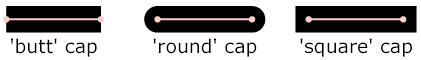
\includegraphics[scale=0.8]{figures/graphics-linecaps}
\end{center}

\tbf{JoinStyle}

Values: \ttt{JOIN\_BEVEL}, \ttt{JOIN\_ROUND}, \ttt{JOIN\_MITER}

This enum indicates the shape to be used when two line segments are joined,
in line or shape figures.

\begin{center}

\includegraphics[scale=0.8]{figures/graphics-linejoins}
\end{center}

\tbf{FillRule}

Values: \ttt{FILL\_EVENODD}, \ttt{FILL\_NONZERO}.

This enum determines which regions of a self-intersecting shape
should be considered to be inside the shape, and thus be filled.

\begin{center}

\includegraphics[scale=0.8]{figures/graphics-fillrule}
\end{center}

\tbf{ArrowHead}

Values: \ttt{ARROW\_NONE}, \ttt{ARROW\_SIMPLE}, \ttt{ARROW\_TRIANGLE}, \ttt{ARROW\_BARBED}.

Some figures support displaying arrowheads at one or both ends of a line.
This enum determines the style of the arrowhead to be used.

\begin{center}

\includegraphics[scale=0.8]{figures/graphics-arrowheads}
\end{center}

\tbf{Interpolation}

Values: \ttt{INTERPOLATION\_NONE}, \ttt{INTERPOLATION\_FAST}, \ttt{INTERPOLATION\_BEST}.

Interpolation is used for rendering an image when it is not displayed at
its native resolution. This enum indicates the algorithm to be used for
interpolation.

The mode \textit{none} selects the "nearest neighbor" algorithm.
\textit{Fast} emphasizes speed, and \textit{best} emphasizes quality;
however, the exact choice of algorithm (bilinear, bicubic, quadratic, etc.)
depends on features of the graphics library that the GUI was implemented with.

\tbf{Anchor}

Values:
\ttt{ANCHOR\_CENTER}, \ttt{ANCHOR\_N}, \ttt{ANCHOR\_E}, \ttt{ANCHOR\_S}, \ttt{ANCHOR\_W},
\ttt{ANCHOR\_NW}, \ttt{ANCHOR\_NE}, \ttt{ANCHOR\_SE}, \ttt{ANCHOR\_SW};
\ttt{ANCHOR\_BASELINE\_START}, \ttt{ANCHOR\_BASELINE\_MIDDLE}, \\ \ttt{ANCHOR\_BASELINE\_END}.

Some figures like text and image figures are placed by specifying a single
point (\textit{position}) plus an anchor mode, a value from this enum. The
anchor mode indicates which point of the bounding box of the figure should
be positioned over the specified point. For example, when using
\ttt{ANCHOR\_N}, the figure is placed so that its top-middle point falls at
the specified point.

The last three, \textit{baseline} constants are only used with text
figures, and indicate that the start, middle or end of the text's baseline
is the anchor point.


\subsection{cLineFigure and Other Figure Classes}

Now the we know all about figures in general, we can look into specific
figure classes.

\subsubsection{Common properties for line figures: cAbstractLineFigure}

\cclass{cAbstractLineFigure} is the common base class for line figures: \cclass{cLineFigure},...TODO

It provides line color, style, width, opacity, and other properties. Lines may
also be augmented with arrowheads at either or both ends.

\begin{itemize}
    \item it has a line color (\ffunc{setLineColor()}/\ffunc{getLineColor()})
    \item it has a line width (\ffunc{setLineWidth()}/\ffunc{getLineWidth()})
    \item it can be partially transparent (\ffunc{setLineOpacity()}/\ffunc{getLineOpacity()})
    \item it can be dashed, dotted, etc. (\ffunc{setLineStyle()}/\ffunc{getLineStyle()})
    \item it can have various line cap styles (butt, square, etc.) (\ffunc{setCapStyle()}/\ffunc{getCapStyle()})
    \item it can have arrowheads at any or both ends (\ffunc{setStartArrowHead()}/\ffunc{getStartArrowHead()}, \ffunc{setEndArrowHead()}/\ffunc{getEndArrowHead()})
    \item it can be chosen whether interactive zoom affects line width (\ffunc{setZoomLineWidth()}/\ffunc{getZoomLineWidth()})
\end{itemize}

Transformations such as scaling or skew do affect the width of the line as it
is rendered on the canvas. Whether zooming (by the user) should also affect
it can be controlled by setting a flag (see setZoomLineWidth()).

The rendering of zero-width lines is currently undefined. It is attempted
to be rendered as a one pixel wide line, regardless of transforms and zoom
level, but it is not possible on all platforms.

\subsubsection{cLineFigure}

\cclass{cLineFigure} displays a single straight line segment. The endpoints
of the line can be set with the \ffunc{setStart()}/\ffunc{setEnd()} methods.

As \cclass{cLineFigure} subclasses from \cclass{cAbstractLineFigure}, it
shares several properties with other line figures:

\subsubsection{cArcFigure}

\cclass{cArcFigure} displays an arc. The arc's geometry is determined by
the bounding box of the circle or ellipse, and a start and end angle. Other
properties such as color and line style are inherited from
\cclass{cAbstractLineFigure}.

\begin{note}
Angles are in radians in the C++ API, but in degrees when the figure is
defined in the NED file via \fprop{@figure}.
\end{note}

getBounds()/setBounds()
getStartAngle()/setStartAngle()
getEndAngle()/setEndAngle()

\subsubsection{cPolylineFigure}

\cclass{cPolylineFigure} displays multiple connecting straight line
segments, or a smoothed curve. The class stores geometry information as a
sequence of points.

The line may be \textit{smoothed}. A smoothed line is drawn
as a series of Bezier curves, which touch the start point of the first
line segment, the end point of the last line segment, and the midpoints
of intermediate line segments, while intermediate points serve as control
points.

Additional properties such as color and line style are inherited from
\cclass{cAbstractLineFigure}.

\begin{cpp} TODO:
        virtual void setPoints(const std::vector<Point>& points);
        virtual int getNumPoints() const {return points.size();}
        virtual const Point& getPoint(int i) const {checkIndex(i); return points[i];}
        virtual void setPoint(int i, const Point& point);
        virtual void addPoint(const Point& point);
        virtual void removePoint(int i);
        virtual void insertPoint(int i, const Point& point);
        virtual bool getSmooth() const {return smooth;}
        virtual void setSmooth(bool smooth);
        virtual JoinStyle getJoinStyle() const {return joinStyle;}
        virtual void setJoinStyle(JoinStyle joinStyle);
\end{cpp}

\subsubsection{cAbstractShapeFigure}

\cclass{cAbstractShapeFigure} is a abstract base class for various shapes,
providing line and fill color, line and fill opacity, line style, line
width, and other properties for them. Both outline and fill are optional.

When the outline is drawn with a width larger than one pixel, it will be
drawn symmetrically, i.e. approximately 50-50% of its width will fall
inside and outside the shape.

Transformations such as scaling or skew do affect the width of the line as it
is rendered on the canvas. Whether zooming (by the user) should also affect
it can be controlled by setting a flag (see setZoomLineWidth()).

The rendering of zero-width lines is currently undefined. It is attempted
to be rendered as a one pixel wide line, regardless of transforms and zoom
level, but it is not possible on all platform.

\subsubsection{cRectangleFigure}

\cclass{cRectangleFigure} displays a rectangle with optionally rounded
corners. As with all shape figures, drawing of both the outline and the
fill are optional. Line and fill color, and several other properties are
inherited from \cclass{cAbstractShapeFigure}.

\subsubsection{cOvalFigure}

\cclass{cOvalFigure} displays a circle or ellipse. As with all shape figures, drawing
of both the outline and the fill are optional. Line and fill color, and
several other properties are inherited from \cclass{cAbstractShapeFigure}.

\subsubsection{cRingFigure}

\cclass{cRingFigure} displays a ring, with explicitly controllable
inner/outer radii. The inner/outer circles (or ellipses) form the outline,
and the area between them is filled. As with all shape figures, drawing of
both the outline and the fill are optional. Line and fill color, and
several other properties are inherited from \cclass{cAbstractShapeFigure}.

\subsubsection{cPieSliceFigure}

\cclass{cPieSliceFigure} displays a pie slice, that is, a section of an
axis-aligned disc or filled ellipse. A pie slice is determined by the
bounding box of the full disc or ellipse, and a start and an end angle. The
outline of the pie slice consists of an arc and two radii. As with all
shape figures, drawing of both the outline and the fill are optional. Line
and fill color, and several other properties are inherited from
cAbstractShapeFigure.

\subsubsection{cPolygonFigure}

\cclass{cPolygonFigure} displays a (closed) polygon, determined by a sequence of points.
The polygon may be \textit{smoothed}. A smoothed polygon is drawn as a series
of cubic Bezier curves, where the curves touch the midpoints of the sides,
and vertices serve as control points. As with all shape figures, drawing of
both the outline and the fill are optional. The drawing of filled self-
intersecting polygons is controlled by the \textit{fill rule} property.
Line and fill color, and several other properties are inherited from
cAbstractShapeFigure.

\subsubsection{cPathFigure}

\cclass{cPathFigure} displays a "path", a complex shape or line modeled after SVG
paths. A path is may consist of any number of straight line segments, Bezier
curves and arcs. The path can be disjoint as well. Closed paths may be filled.
The drawing of filled self-intersecting polygons is controlled by the
\textit{fill rule} property. Line and fill color, and several other properties
are inherited from \cclass{cAbstractShapeFigure}.

The path may be specified with a string similar to an SVG path, or assembled
by calling methods that append new segments (straight lines, arcs or Bezier
curves) to the existing path.

\subsubsection{cAbstractTextFigure}

\cclass{cAbstractTextFigure} is an abstract base class for figures that
display text. Text may be multi-line. Font, color, opacity, position and
anchoring are specified in this class.

\subsubsection{cTextFigure}

\cclass{cTextFigure} displays text which is affected by zooming and
transformations. Font, color, position, anchoring and other properties are
inherited from \cclass{cAbstractTextFigure}.

\subsubsection{cLabelFigure}

\cclass{cLabelFigure} displays text which is unaffected by zooming or
transformations, except its position. Font, color, position, anchoring and
other properties are inherited from \cclass{cAbstractTextFigure}.

\subsubsection{cAbstractImageFigure}

\cclass{cAbstractImageFigure} is an abstract base class for image figures.

The location of the image on the canvas is determined jointly by the
\textit{position} and \textit{anchor} properties. The anchor tells how to
position the image relative to the positioning point. For example,
if anchor is \ttt{ANCHOR\_CENTER} then the image is centered on the point;
if anchor is \ttt{ANCHOR\_N} then the image will be drawn so that its top center
point is at the positioning point. Anchor defaults to \ttt{ANCHOR\_CENTER}.

Images may be drawn at their "natural" size, or may be scaled to a
specified size by setting the width and/or height properties. One can
choose from several interpolation modes that control how the image is
rendered. Interpolation defaults to \ttt{INTERPOLATION\_FAST}.

Images can be tinted; this feature is controlled by a tint color and
a tint amount, a [0,1] real number.

Images may be rendered as partially transparent, which is controlled
by the opacity property, a [0,1] real number. (The rendering process
will combine this property with the transparency information contained
within the image, i.e. the alpha channel.)

\subsubsection{cImageFigure}

\cclass{cImageFigure} displays an image, typically an icon or a background image,
loaded from the {\opp} image path. Positioning and other properties
are inherited from \cclass{cAbstractImageFigure}.

\subsubsection{cIconFigure}

\cclass{cIconFigure} displays a non-zooming image, loaded from the {\opp}
image path. Positioning and other properties are inherited from
cAbstractImageFigure.

\cclass{cIconFigure} not affected by transforms or zoom, except its position.

\subsubsection{cPixmapFigure}

\cclass{cPixmapFigure} displays a user-defined raster image. A pixmap
figure may be used to display e.g. a heat map. Support for scaling and
various interpolation modes are useful here. Positioning and other
properties are inherited from \cclass{cAbstractImageFigure}.

\subsubsection{cGroupFigure}

\cclass{cGroupFigure} is for the sole purpose of grouping its children. It
has no visual appearance. The usefulness of a group figure comes from the
fact that elements of a group can be hidden / shown together, and also
transformations are inherited from parent to child, thus, children of a
group can be moved, scaled, rotated, etc. together by updating the group's
transformation matrix.


\subsection{Defining New Figure Types}

There are two ways the set of figure type can be extended:

\begin{enumerate}
  \item Compound figures.
  \item New standalone figure types
\end{enumerate}

Compound figures are useful when the graphical presentation of a simulation
grows complex, and it becomes desirable to be able to group certain figures
into larger units that can be created and manipulated like a single figure.

Such compound figures can be created by subclassing e.g. \cclass{cGroupFigure}.
The constructor would create and add subfigures as children, and also remember
their pointers. Added getter and setter methods would delegate to subfigures.

It is is more difficult to create new figure types where the rendering is not
based on already existing figures. The difficulty arises from the point that
figures are only data storate classes, actual drawing takes place in the
GUI library such as Tkenv and Qtenv. Thus, it is not enough to write the new
figure class itself, but one also needs to extend Tkenv and/or Qtenv as well,
to add the rendering code.

We won't go into full details of how to extend Tkenv/Qtenv here, just give
a few pointers in case you wanted to do that.

In both Tkenv and Qtenv, rendering is done with the help of figure renderer
classes that have a class hierarchy roughly parallel to the
\cclass{cFigure} inheritance tree. The bases classes are incidentally
called \cclass{FigureRenderer}. How figure renderers do their job is
different in Tkenv and Qtenv: in Tkenv, rendering occurs by creating and
maintaining Tkpath graphics items on a Tkpath canvas; on Qtenv, they create
and manipulate \cclass{QGraphicsItem}s on a \cclass{QGraphicsView}.
To create a new figure type, one likely needs to create their own
\cclass{FigureRenderer} subclass, and add it into Tkenv/Qtenv.

The way renderer classes are associated with figure classes is tricky. TODO


\section{3D Visualization}
\label{sec:ch-graphics:osg}

\subsection{OpenSceneGraph and osgEarth}

{\opp}'s 3D visualization is based on OpenSceneGraph and osgEarth. These
libraries offer high-level functionality, such as reading 3D model files
directly, or accessing online map and satellite imagery data sources, and
displaying them as maps, 3D terrain or globe.

OpenSceneGraph (openscenegraph.org), or OSG for short, is the base library.
It is best to quote their web site:

\begin{displayquote}
"OpenSceneGraph is an open source high performance 3D graphics toolkit,
used by application developers in fields such as visual simulation, games,
virtual reality, scientific visualization and modeling. Written entirely in
Standard C++ and OpenGL, it runs on all Windows platforms, OS X, GNU/Linux,
IRIX, Solaris, HP-UX, AIX and FreeBSD operating systems. OpenSceneGraph is
now well established as the world leading scene graph technology, used
widely in the vis-sim, space, scientific, oil-gas, games and virtual
reality industries."
\end{displayquote}

In turn, osgEarth (osgearth.org) is a geospatial SDK and terrain engine built on top
of OpenSceneGraph, not quite unlike Google Earth. It has many attractive features:

\begin{itemize}
\item Able to use various street map providers, satellite imaging providers, altitude data sources, both online and offline
\item Data from online sources may be exported into a file suitable for offline use
\item Scene may be annotated with various types of graphical objects
\item Includes conversion between various geographical coordinate systems
\end{itemize}

On the basic level, osgEarth is very easy to use. To get started, one only
needs to create a simple XML file, and point it at the appropriate map data
source.

Using OSG and osgEarth, one can build 3D visualization for a wide range of
simulations involving terrains, roads, urban environments, indoor
environments, satellites, and more. Considering wireless network
simulations, for example, one can create a scene that displays mobile nodes,
transmission ranges, connectivity graphs, statistics, wireless transmissions, etc.

\subsection{OpenScenegraph in {\opp}}

3D visualization is separate from display string based and canvas.

Models have no built-in visualization, 3D scenes have to
be built by the simulation programmer, and they also appear on a separate
GUI area.

For 3D visualization, {\opp} basically exposes the OpenSceneGraph API.
You assemble an OSG scene graph in the model, and give it to {\opp} for
display. The scene graph can be updated at runtime, and changes will be
reflected in the display.

The central {\opp} class is \cclass{cOsgCanvas}. \cclass{cOsgCanvas}.
wraps a scene graph, plus hints such as default camera position.
Every module has a built-in \cclass{cOsgCanvas}, which is created on demand.

Additional \cclass{cOsgCanvas} instances may be created.

only in Qtenv.

\begin{note}
The OSG viewer is part of the GUI library, Qtenv, and it is \textit{not}
directly accessible from models.
\end{note}

\subsection{Code}

Model code should surround OSG-specific code with \#ifdef HAVE\_OSG

Example code:

"Glider" demo:

\begin{cpp}
#include <osgDB/ReadFile>
#include <omnetpp.h>
...
void DemoModule::initialize() {
    osg::Node *scene = osgDB::readNodeFile("glider.osgb");
    cOsgCanvas *osgCanvas = getParentModule()->getOsgCanvas();
    osgCanvas->setScene(scene); // the scene graph
    osgCanvas->setClearColor(cOsgCanvas::Color(0,0,64)); // hint
}
\end{cpp}

"Boston" demo:
 substitute "boston.earth" for "glider.osgb"
 add the following line:

\begin{cpp}
osgCanvas->setViewerStyle(cOsgCanvas::STYLE_EARTH);
\end{cpp}

Everything else is achieved by manipulating the scene graph via the OSG API.

\subsection{Tips}

some starting points:
osg files
transforms
animations

look at the sample simulations
TODO


\section{refreshDisplay()}
\label{sec:ch-graphics:refreshdisplay}

\ffunc{refreshDisplay()} is a method that is called on all components of
the simulation by graphical user interfaces (Qtenv, Tkenv) whenever GUI
contents need to be refreshed, such as after network setup, after
processing some simulation events, or before and after finalization.
Components that contain visualization-related code are expected to override
\ffunc{refreshDisplay()}, and move visualization code display string
manipulation, canvas figures maintenance, OSG scene graph update, etc.)
into it.

As it is unpredictable when and whether this method is invoked, the
simulation logic should not depend on it. It is advisable that code in
\ffunc{refreshDisplay()} does not alter the state of the model at all. This
behavior is gently encouraged by having this method declared as const.
(Data members that do need to be updated inside \ffunc{refreshDisplay()}, i.e.
those related to visualization, may be declared mutable to allow that).

Tkenv and Qtenv invoke \ffunc{refreshDisplay()} with similar strategies: in Step
and Run mode, after each event; in Fast Run and Express Run mode, every
time the screen is refereshed, which is typically on the order of once
per second. Cmdenv does not invoke \ffunc{refreshDisplay()} at all.

Note that overriding \ffunc{refreshDisplay()} is generally preferable to doing
display updates as part of event handling: it results in essentially
zero per-event runtime overhead, and potentially more consistent
information being displayed (as all components refresh their visualization,
not only the one which has just processed an event.)

\begin{cpp}
virtual void refreshDisplay() const;
\end{cpp}


TODO

%%% Local Variables:
%%% mode: latex
%%% TeX-master: "usman"
%%% End:

